\documentclass[14pt, fleqn, paper=letter, oneside]{scrartcl}

\newcommand{\includehead}{false}
\newcommand{\includefoot}{false}

% set basic page format
\usepackage[headsepline=\includehead, footsepline=\includefoot]{scrlayer-scrpage} 
\usepackage[margin=0.375in,
    footskip=1.5\baselineskip,
    headsep=0.5\baselineskip,
    includehead=\includehead, includefoot=\includefoot]{geometry}   %Fixed margins
\usepackage[compact]{titlesec}

%\usepackage{setspace}
%\onehalfspace
%\doublespace    

% image support
\renewcommand{\topfraction}{0.85}   %Fixes float spacing
\renewcommand{\textfraction}{0.1}
\renewcommand{\floatpagefraction}{0.75}
\usepackage{graphicx}
	\graphicspath{{/Users/fred/Library/TeXShop/Images/}{./Images/}}
\usepackage[space]{grffile}		

% symbol support
\usepackage{siunitx}    %SI unit : \si{\'unit'} or \SI{#}{\'unit'}
\sisetup{detect-all}
\usepackage{chemfig}    %Write chemical formulas
\usepackage{mathtools}  %Basic math an extension of amsmath

% formatting support
\usepackage{multicol}   %Multiple cols body : command \multicols{#}{'text'}
\usepackage{multirow}   %Multiple row spanning in tables : \multirow{#}{width}{'text'}
\usepackage{enumitem}   %Enumeration control
\usepackage{hyperref} % hyperlinks
\usepackage{soul} % highlighting with \hl{command}
\usepackage{tabularx}


% font and date format
\usepackage{newtxtext}
\setkomafont{disposition}{\bfseries}
\usepackage{fancyref}           %Automatically adds Table (tab:' ') or Figure (fig:' ')
\usepackage{texdate}
\initcurrdate
\def\setdateformat{e\ b\ y\ }
\renewcommand{\headfont}{\normalfont}
\renewcommand{\footfont}{\normalfont}

% useful commands
\newcommand{\biu}[1]{\textbf{\emph{\underline{#1}}}}
\newcommand{\centerframe}[1]{ % this command makes a box around the content
    {\centering\fbox{\begin{minipage}{0.975\columnwidth}#1\end{minipage}}}}

% document commands
%\ihead{Name:}
%\chead{Hour:}
%\ohead{Date:}
%\ifoot{Revised \printdate}
%\cfoot{\maintitle}
%\ofoot{\thepage}
\newcommand{\maintitle}{The Author}

%===================================
\begin{document}
\begin{table}[h]
\renewcommand{\arraystretch}{2.5}
\centering
\begin{tabularx}{\textwidth}{|c|X|X|X|}
\hline
  & Observation
  & Your Inference
  & Partners Inference 
\\\hline
  & The ground is wet.                                                                                                              & It must have rained last night.                                                                                                                     & They must have watered their lawn.                  \\ \hline
1 &                                                                                                                                 &                                                                                                                                                     &                                                     \\ \hline
2 &&&\\ \hline
3 &&&\\ \hline
4 &&&\\ \hline
5 &&&\\ \hline
6 &&&\\ \hline
7 &&&\\ \hline
8 &&&\\ \hline
9 &&&\\ \hline
10 &&&\\ \hline
\end{tabularx}
\end{table}

\textbf{Folding instructions}
Fold like the image below to cover up your inferences when you pass to your partner.

\begin{figure}[h]
\centering
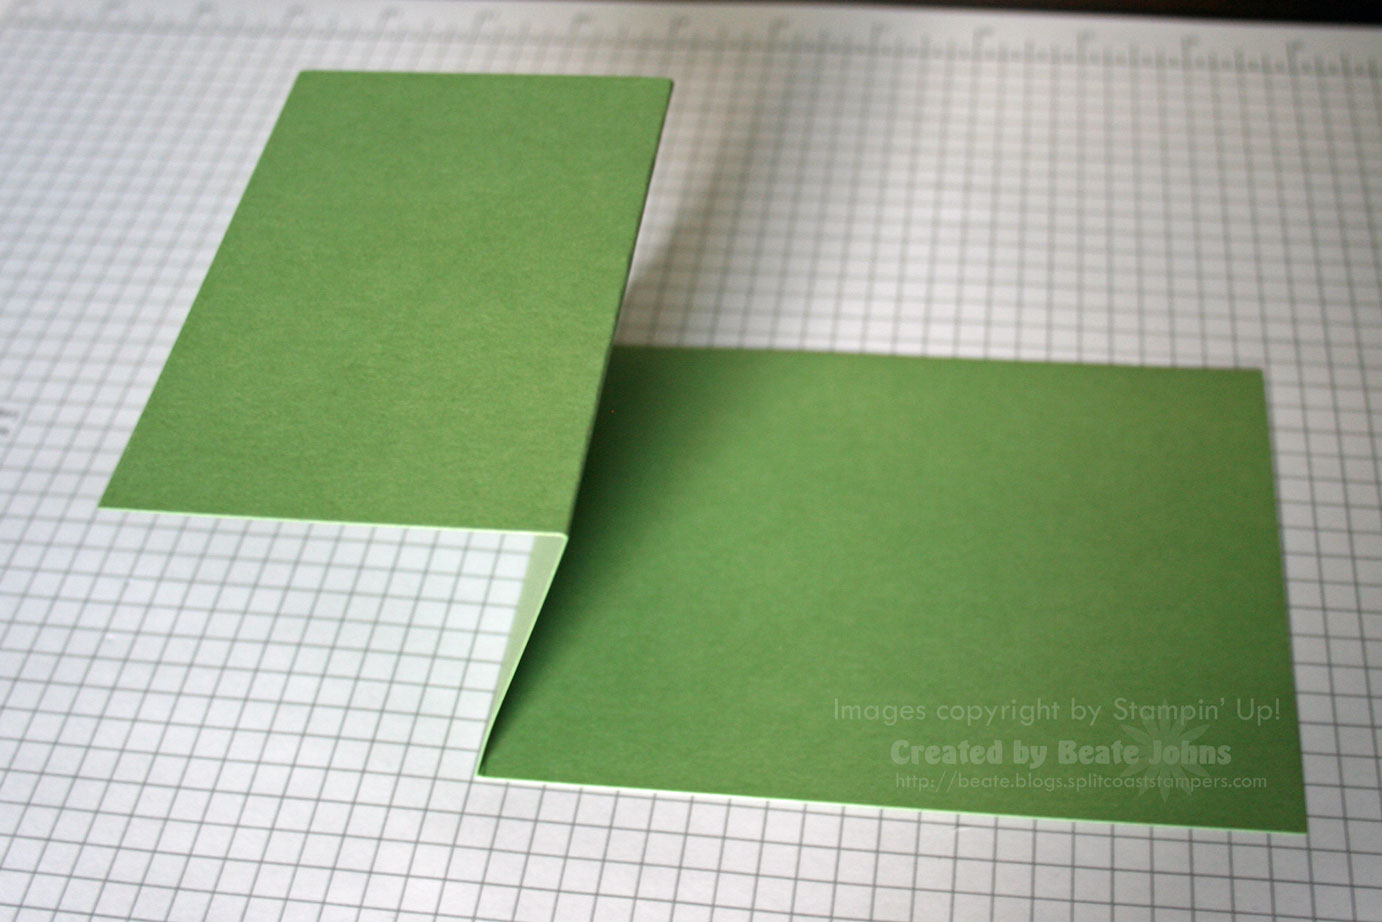
\includegraphics[height=30mm]{fold}

\end{figure}






































\end{document}